\documentclass[11pt,a4paper]{report}
\usepackage[textwidth=37em,vmargin=30mm]{geometry}
\usepackage{calc,xunicode,amsmath,amssymb,paralist,enumitem,tabu,booktabs,datetime2,xeCJK,xeCJKfntef,listings}
\usepackage{tocloft,fancyhdr,tcolorbox,xcolor,graphicx,eso-pic,xltxtra,xelatexemoji}

\newcommand{\envyear}[0]{2025}
\newcommand{\envdatestr}[0]{2025-03-24}
\newcommand{\envfinaldir}[0]{webdb/2025/20250324/final}

\usepackage[hidelinks]{hyperref}
\hypersetup{
    colorlinks=false,
    pdfpagemode=FullScreen,
    pdftitle={Web Digest - \envdatestr}
}

\setlength{\cftbeforechapskip}{10pt}
\renewcommand{\cftchapfont}{\rmfamily\bfseries\large\raggedright}
\setlength{\cftbeforesecskip}{2pt}
\renewcommand{\cftsecfont}{\sffamily\small\raggedright}

\setdefaultleftmargin{2em}{2em}{1em}{1em}{1em}{1em}

\usepackage{xeCJK,xeCJKfntef}
\xeCJKsetup{PunctStyle=plain,RubberPunctSkip=false,CJKglue=\strut\hskip 0pt plus 0.1em minus 0.05em,CJKecglue=\strut\hskip 0.22em plus 0.2em}
\XeTeXlinebreaklocale "zh"
\XeTeXlinebreakskip = 0pt


\setmainfont{Brygada 1918}
\setromanfont{Brygada 1918}
\setsansfont{IBM Plex Sans}
\setmonofont{JetBrains Mono NL}
\setCJKmainfont{Noto Serif CJK SC}
\setCJKromanfont{Noto Serif CJK SC}
\setCJKsansfont{Noto Sans CJK SC}
\setCJKmonofont{Noto Sans CJK SC}

\setlength{\parindent}{0pt}
\setlength{\parskip}{8pt}
\linespread{1.15}

\lstset{
	basicstyle=\ttfamily\footnotesize,
	numbersep=5pt,
	backgroundcolor=\color{black!5},
	showspaces=false,
	showstringspaces=false,
	showtabs=false,
	tabsize=2,
	captionpos=b,
	breaklines=true,
	breakatwhitespace=true,
	breakautoindent=true,
	linewidth=\textwidth
}






\newcommand{\coverpic}[2]{
    % argv: itemurl, authorname
    Cover photo by #2~~(\href{#1}{#1})
}
\newcommand{\makeheader}[0]{
    \begin{titlepage}
        % \newgeometry{hmargin=15mm,tmargin=21mm,bmargin=12mm}
        \begin{center}
            
            \rmfamily\scshape
            \fontspec{BaskervilleF}
            \fontspec{Old Standard}
            \fontsize{59pt}{70pt}\selectfont
            WEB\hfill DIGEST
            
            \vfill
            % \vskip 30pt
            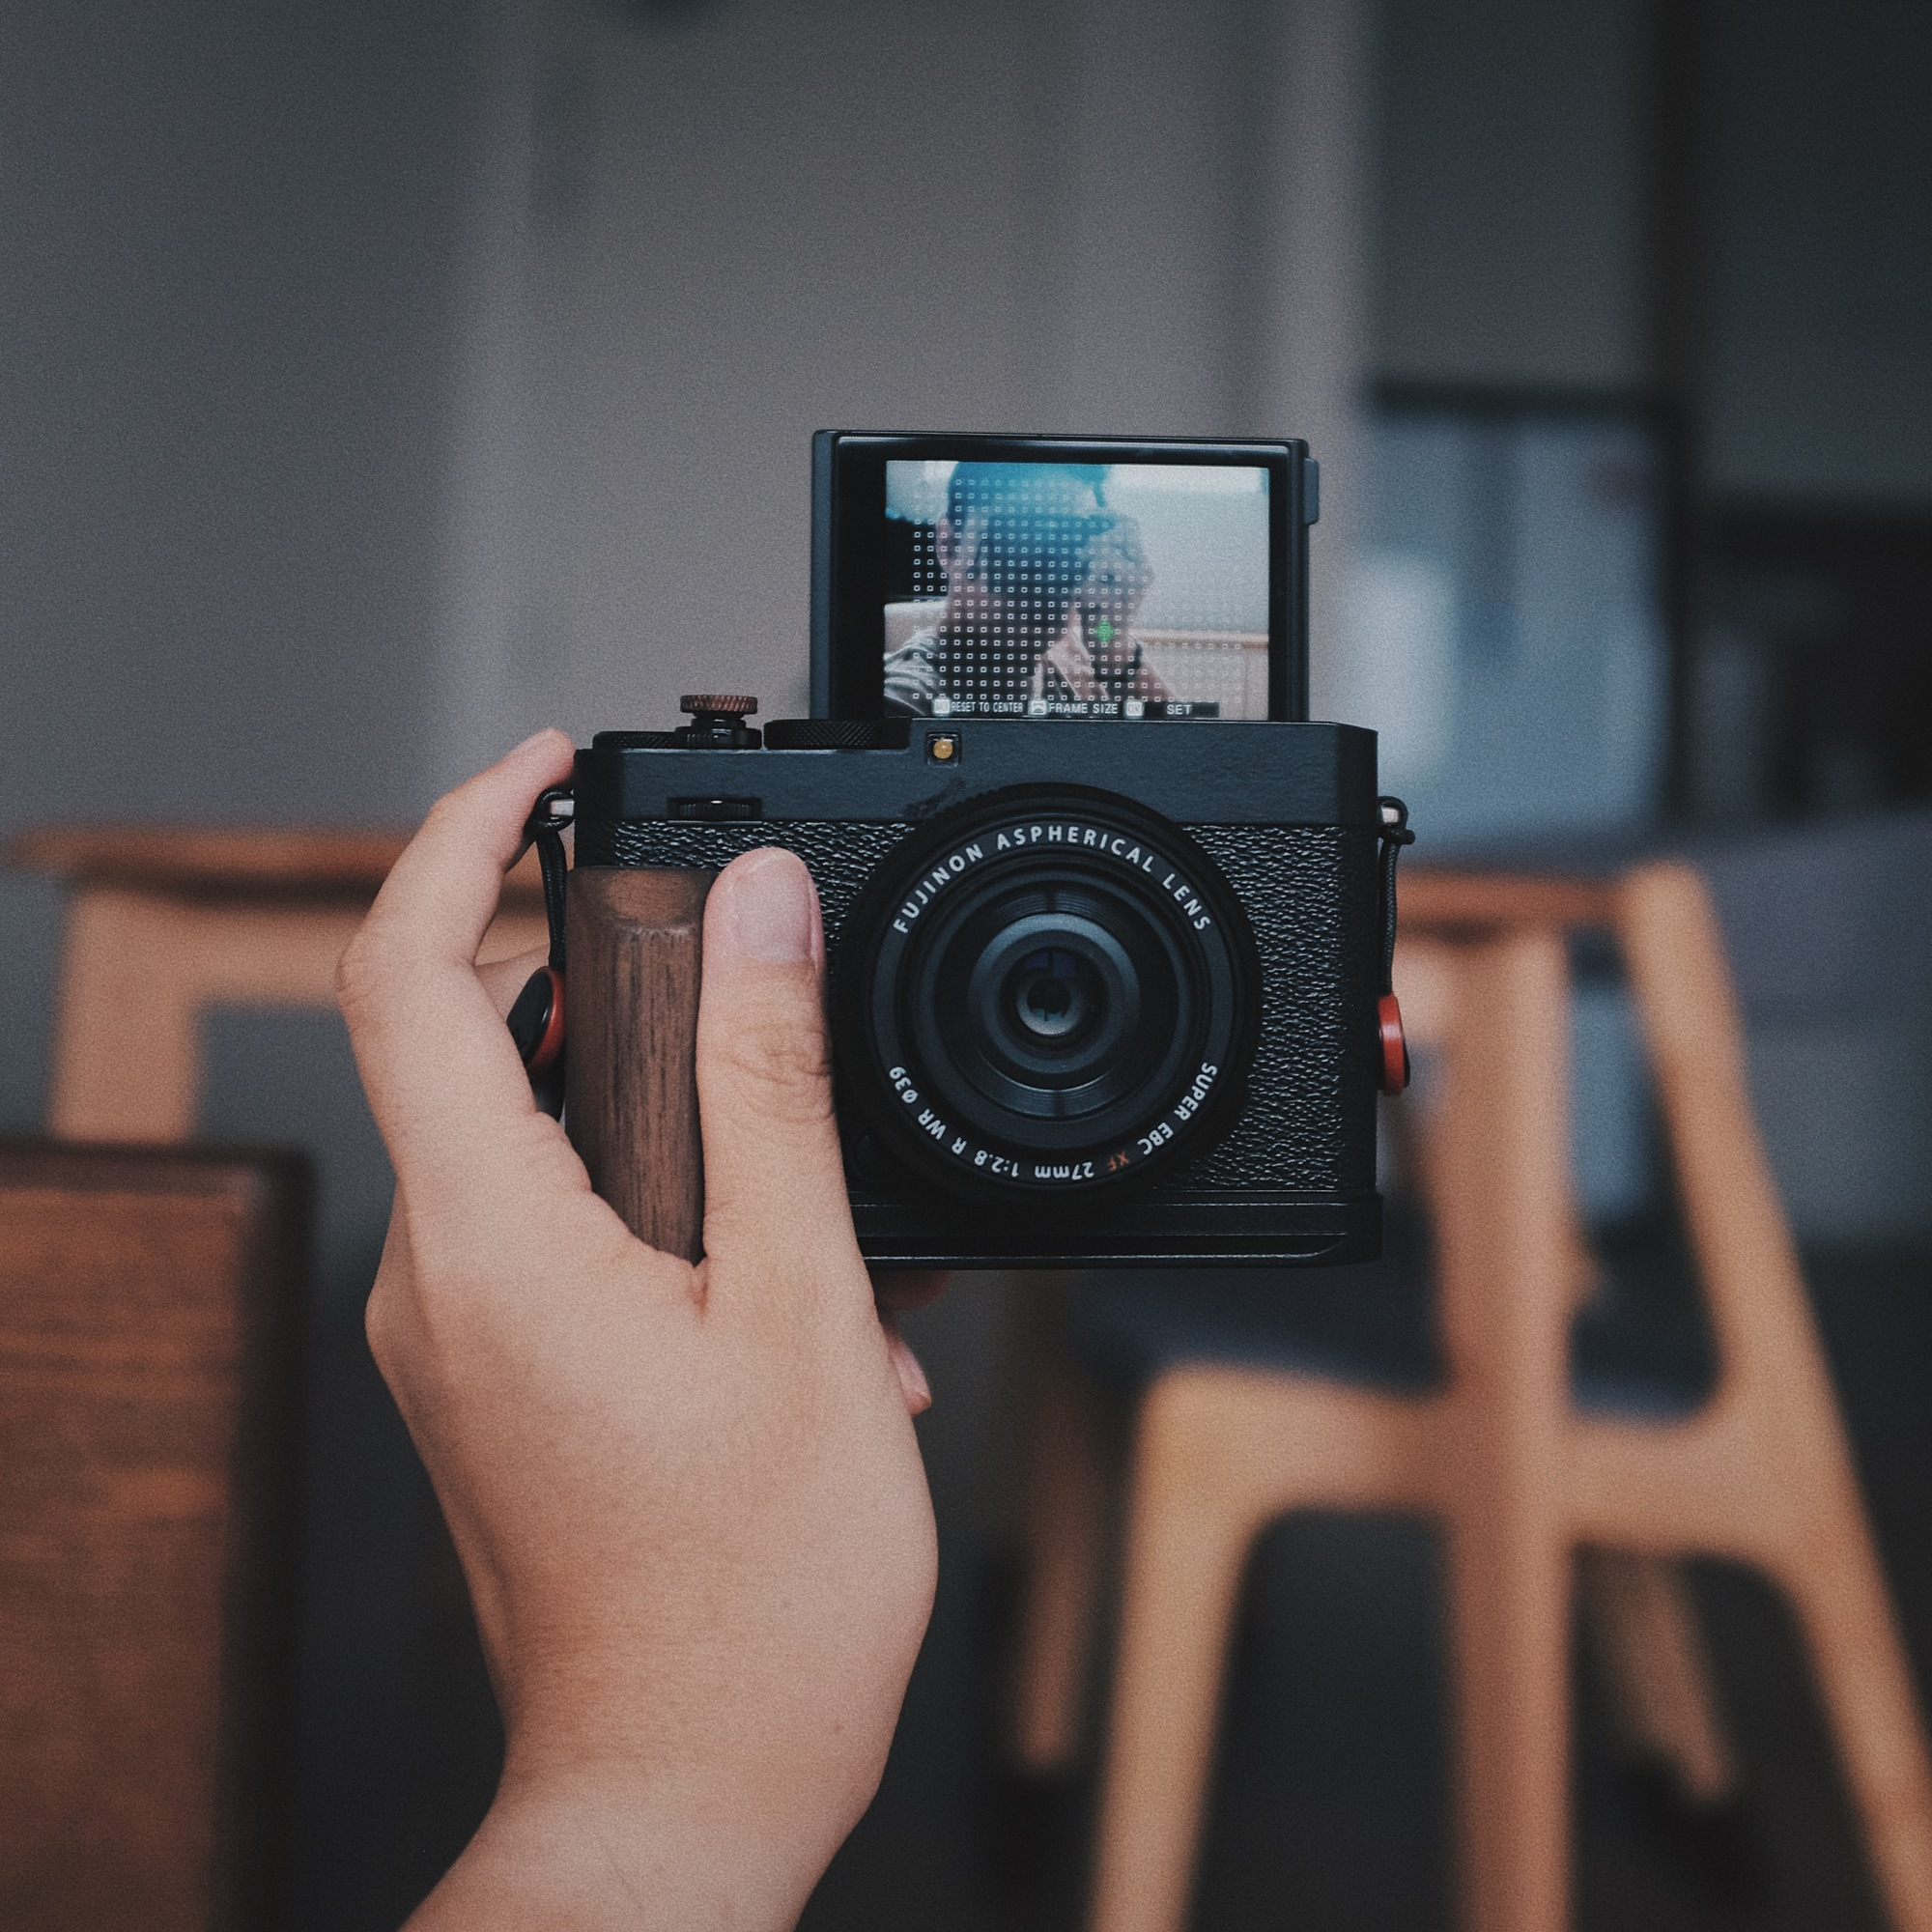
\includegraphics[width=\linewidth]{\envfinaldir/coverpic-prod.jpg}\par
            % \vskip 30pt
            \vfill

            \normalsize\rmfamily\scshape
            \copyright{} The Web Digest Project \hfill\large \envdatestr
        \end{center}
    \end{titlepage}
    % \restoregeometry
}
\newcommand{\simplehref}[1]{%
    \textcolor{blue!80!green}{\href{#1}{#1}}%
}
\renewcommand{\contentsname}{\center\Huge\sffamily\bfseries Contents\par\vskip 20pt}
\newcounter{ipartcounter}
\setcounter{ipartcounter}{0}
\newcommand{\ipart}[1]{
    % \vskip 20pt
    \clearpage
    \stepcounter{ipartcounter}
    \phantomsection
    \addcontentsline{toc}{chapter}{#1}
    % \begin{center}
    %     \Huge
    %     \sffamily\bfseries
    %     #1
    % \end{center}
    % \vskip 20pt plus 7pt
}
\newcounter{ichaptercounter}
\setcounter{ichaptercounter}{0}
\newcommand{\ichapter}[1]{
    % \vskip 20pt
    \clearpage
    \stepcounter{ichaptercounter}
    \phantomsection
    \addcontentsline{toc}{section}{\numberline{\arabic{ichaptercounter}}#1}
    \begin{center}
        \Huge
        \sffamily\bfseries
        #1
    \end{center}
    \vskip 20pt plus 7pt
}
\newcommand{\entrytitlefont}[1]{\subsection*{\raggedright\Large\sffamily\bfseries#1}}
\newcommand{\entryitemGeneric}[2]{
    % argv: title, url
    \parbox{\linewidth}{
        \entrytitlefont{#1}\par\vskip 5pt
        \footnotesize\ttfamily\mdseries
        \simplehref{#2}
    }\vskip 11pt plus 11pt minus 1pt
}
\newcommand{\entryitemGithub}[3]{
    % argv: title, url, desc
    \parbox{\linewidth}{
        \entrytitlefont{#1}\par\vskip 5pt
        \footnotesize\ttfamily\mdseries
        \simplehref{#2}\par\vskip 5pt
        \small\rmfamily\mdseries#3
    }\vskip 11pt plus 11pt minus 1pt
}
\newcommand{\entryitemAp}[3]{
    % argv: title, url, desc
    \parbox{\linewidth}{
        \entrytitlefont{#1}\par\vskip 5pt
        \footnotesize\ttfamily\mdseries
        \simplehref{#2}\par\vskip 5pt
        \small\rmfamily\mdseries#3
    }\vskip 11pt plus 11pt minus 1pt
}
\newcommand{\entryitemHackernews}[3]{
    % argv: title, hnurl, rawurl
    % \parbox{\linewidth}{
    %     \entrytitlefont{#1}\par\vskip 5pt
    %     \footnotesize\ttfamily\mdseries
    %     \simplehref{#3}\par
    %     \textcolor{black!50}{\href{#2}{#2}}
    % }\vskip 11pt plus 11pt minus 1pt
    \begin{minipage}{\linewidth}
            \entrytitlefont{#1}\par\vskip 5pt
            \footnotesize\ttfamily\mdseries
            \simplehref{#3}\par
            \textcolor{black!50}{\href{#2}{#2}}
    \end{minipage}\par\vskip 11pt plus 11pt minus 1pt
}







\begin{document}

\makeheader

\tableofcontents\clearpage




\ipart{Developers}
\ichapter{Hacker News}
\entryitemTwoLinks{Show HN: My iOS app to practice sight reading (10 years in the App Store)}{https://news.ycombinator.com/item?id=43456030}{https://apps.apple.com/us/app/notes-sight-reading-trainer/id874386416}

\entryitemTwoLinks{Show HN: LinkedIn sucks, so I built a better one}{https://news.ycombinator.com/item?id=43454915}{https://heyopenspot.com/}

\entryitemTwoLinks{A USB Interface to the "Mother of All Demos" Keyset}{https://news.ycombinator.com/item?id=43453582}{https://www.righto.com/2025/03/mother-of-all-demos-usb-keyset-interface.html}

\entryitemTwoLinks{Technicalities of Homeworld 2 Backgrounds}{https://news.ycombinator.com/item?id=43452688}{https://simonschreibt.de/gat/homeworld-2-backgrounds/}

\entryitemTwoLinks{The Worst Programmer I Know (2023)}{https://news.ycombinator.com/item?id=43452649}{https://dannorth.net/the-worst-programmer/}

\entryitemTwoLinks{Show HN: I built website for sharing Drum Patterns}{https://news.ycombinator.com/item?id=43452629}{http://drumpatterns.onether.com}

\entryitemTwoLinks{argp: GNU-style command line argument parser for Go}{https://news.ycombinator.com/item?id=43452525}{https://github.com/tdewolff/argp}

\entryitemTwoLinks{Is it safe to travel to the United States with your phone?}{https://news.ycombinator.com/item?id=43452474}{https://www.theverge.com/policy/634264/customs-border-protection-search-phone-airport-rights}

\entryitemTwoLinks{The SeL4 Microkernel: An Introduction [pdf]}{https://news.ycombinator.com/item?id=43452185}{https://sel4.systems/About/seL4-whitepaper.pdf}

\entryitemTwoLinks{The case of the critical section that let multiple threads enter a block of code}{https://news.ycombinator.com/item?id=43451525}{https://devblogs.microsoft.com/oldnewthing/20250321-00/?p=110984}

\entryitemTwoLinks{Do viruses trigger Alzheimer's?}{https://news.ycombinator.com/item?id=43451397}{https://www.economist.com/science-and-technology/2025/03/17/do-viruses-trigger-alzheimers}

\entryitemTwoLinks{Improving recommendation systems and search in the age of LLMs}{https://news.ycombinator.com/item?id=43450732}{https://eugeneyan.com/writing/recsys-llm/}

\entryitemTwoLinks{Next.js version 15.2.3 has been released to address a security vulnerability}{https://news.ycombinator.com/item?id=43448723}{https://nextjs.org/blog/cve-2025-29927}

\entryitemTwoLinks{CEO of Kubient sentenced for fraud}{https://news.ycombinator.com/item?id=43448606}{https://arstechnica.com/gadgets/2025/03/ceo-of-ai-ad-tech-firm-pledging-world-free-of-fraud-sentenced-for-fraud/}

\entryitemTwoLinks{Quitting an Intel x86 Hypervisor}{https://news.ycombinator.com/item?id=43448457}{https://halobates.de/blog/p/446}

\entryitemTwoLinks{``Vibe Coding'' vs. Reality}{https://news.ycombinator.com/item?id=43448432}{https://cendyne.dev/posts/2025-03-19-vibe-coding-vs-reality.html}

\entryitemTwoLinks{Mathematical Methods for Physics [pdf]}{https://news.ycombinator.com/item?id=43448193}{https://www.ma.imperial.ac.uk/~dturaev/Mathematical\_Methods2021.pdf}

\entryitemTwoLinks{Italy demands Google poison DNS under strict Piracy Shield law}{https://news.ycombinator.com/item?id=43448112}{https://arstechnica.com/gadgets/2025/03/italian-court-orders-google-to-block-iptv-pirate-sites-at-dns-level/}

\entryitemTwoLinks{NixOS and reproducible builds could have detected the xz backdoor}{https://news.ycombinator.com/item?id=43448075}{https://luj.fr/blog/how-nixos-could-have-detected-xz.html}

\entryitemTwoLinks{The polar vortex is hitting the brakes}{https://news.ycombinator.com/item?id=43448023}{https://www.climate.gov/news-features/blogs/polar-vortex/polar-vortex-hitting-brakes}\ichapter{Phoronix}
\entryitemGeneric{\hskip 0pt{}EROFS Being Extended To Handle Massive Amounts Of Data For AI Model Training}{https://www.phoronix.com/news/Linux-6.15-EROFS}

\entryitemGeneric{\hskip 0pt{}Hyprland 0.48 Adds A "Application Not Responding" Dialog, Better Color Management}{https://www.phoronix.com/news/Hyprland-0.48-Released}

\entryitemGeneric{\hskip 0pt{}Arch Linux Powered Endeavour OS "Mercury Neo" Released}{https://www.phoronix.com/news/Endeavour-OS-Mercury-Neo}

\entryitemGeneric{\hskip 0pt{}LLVM/Clang Compiler Being Adapted For AVX10.2 Now Making 512-bit Support Mandatory}{https://www.phoronix.com/news/LLVM-Clang-AVX10.2-Always-512}

\entryitemGeneric{\hskip 0pt{}Qualcomm Iris Video Decode Driver \& DesignWare HDMI Input Support Ready For Linux 6.15}{https://www.phoronix.com/news/Linux-6.15-Media-Subsystem}

\entryitemGeneric{\hskip 0pt{}Rust Additions For GCC 15 Bring Support For if-let Statements, Other Improvements}{https://www.phoronix.com/news/GCC-15-Rust-if-let}

\entryitemGeneric{\hskip 0pt{}Sched\_Ext Changes Submitted For Linux 6.15}{https://www.phoronix.com/news/Linux-6.15-Sched-Ext}

\entryitemGeneric{\hskip 0pt{}FreeDesktop.org GitLab Transitions To New Server Infrastructure}{https://www.phoronix.com/news/FreeDesktop-GitLab-On-Hetzner}

\entryitemGeneric{\hskip 0pt{}Linux 6.15 Plans To Drop Support For A Useless CRC-32 Checksum In The Kernel Image}{https://www.phoronix.com/news/Linux-6.15-Drop-Useless-CRC-32}\ichapter{Dribbble}
\entryitemGeneric{\hskip 0pt{}PurePaws - Logo Design}{https://dribbble.com/shots/25797575-PurePaws-Logo-Design}

\entryitemGeneric{\hskip 0pt{}Central Coast}{https://dribbble.com/shots/25794367-Central-Coast}

\entryitemGeneric{\hskip 0pt{}S mark}{https://dribbble.com/shots/25796446-S-mark}

\entryitemGeneric{\hskip 0pt{}The Sequencer Poster}{https://dribbble.com/shots/25798231-The-Sequencer-Poster}

\entryitemGeneric{\hskip 0pt{}Puzzle Fintech UI/UX design, User Interface experience}{https://dribbble.com/shots/25652036-Puzzle-Fintech-UI-UX-design-User-Interface-experience}

\entryitemGeneric{\hskip 0pt{}Sidebar Navigation for Core 2.0 – Dashboard Builder}{https://dribbble.com/shots/25790810-Sidebar-Navigation-for-Core-2-0-Dashboard-Builder}

\entryitemGeneric{\hskip 0pt{}Novascan}{https://dribbble.com/shots/25790443-Novascan}

\entryitemGeneric{\hskip 0pt{}Plain - Branding}{https://dribbble.com/shots/25790107-Plain-Branding}

\entryitemGeneric{\hskip 0pt{}Halo Movie poster}{https://dribbble.com/shots/25791667-Halo-Movie-poster}

\entryitemGeneric{\hskip 0pt{}Mixed Stickers}{https://dribbble.com/shots/25737407-Mixed-Stickers}

\entryitemGeneric{\hskip 0pt{}Decades of Unforgettable Hits}{https://dribbble.com/shots/25792477-Decades-of-Unforgettable-Hits}

\entryitemGeneric{\hskip 0pt{}Crypto Bridge}{https://dribbble.com/shots/25783744-Crypto-Bridge}

\entryitemGeneric{\hskip 0pt{}Eclipse - Logo Design}{https://dribbble.com/shots/25784396-Eclipse-Logo-Design}

\entryitemGeneric{\hskip 0pt{}Cargo Shipment App UI}{https://dribbble.com/shots/25784159-Cargo-Shipment-App-UI}

\entryitemGeneric{\hskip 0pt{}Burn Bright, Take Flight}{https://dribbble.com/shots/25778930-Burn-Bright-Take-Flight}

\entryitemGeneric{\hskip 0pt{}Core 2.0 – Dashboard Builder}{https://dribbble.com/shots/25782776-Core-2-0-Dashboard-Builder}

\entryitemGeneric{\hskip 0pt{}The Planner app}{https://dribbble.com/shots/25769751-The-Planner-app}

\entryitemGeneric{\hskip 0pt{}PieLabs Unused Logo Design}{https://dribbble.com/shots/25784372-PieLabs-Unused-Logo-Design}

\entryitemGeneric{\hskip 0pt{}Mammut Logo Redesign Concept}{https://dribbble.com/shots/25776663-Mammut-Logo-Redesign-Concept}

\entryitemGeneric{\hskip 0pt{}Cimet Logo Grid}{https://dribbble.com/shots/25710567-Cimet-Logo-Grid}

\entryitemGeneric{\hskip 0pt{}Bento grid \& dashboard for revops startup}{https://dribbble.com/shots/25765472-Bento-grid-dashboard-for-revops-startup}

\entryitemGeneric{\hskip 0pt{}Glide wallet}{https://dribbble.com/shots/25768771-Glide-wallet}

\entryitemGeneric{\hskip 0pt{}DL}{https://dribbble.com/shots/25775198-DL}

\entryitemGeneric{\hskip 0pt{}bigbeardamian: Badge Design}{https://dribbble.com/shots/25737398-bigbeardamian-Badge-Design}


\ipart{Developers~~~~(zh-Hans)}
\ichapter{Solidot}
\entryitemGeneric{\hskip 0pt{}俄测试网络主权,完全切断 Cloudflare 连接}{https://www.solidot.org/story?sid=80858}

\entryitemGeneric{\hskip 0pt{}休闲游戏增加老年人的幸福感}{https://www.solidot.org/story?sid=80857}

\entryitemGeneric{\hskip 0pt{}意大利要求 Google DNS 服务器修改盗版网站的 DNS 解析}{https://www.solidot.org/story?sid=80856}

\entryitemGeneric{\hskip 0pt{}AMD 推出在本地运行大模型的开源项目 Gaia }{https://www.solidot.org/story?sid=80855}

\entryitemGeneric{\hskip 0pt{}微软通过电子邮件建议 Windows 10 用户购买新 PC}{https://www.solidot.org/story?sid=80854}

\entryitemGeneric{\hskip 0pt{}雅虎将 TechCrunch 出售给 Regent}{https://www.solidot.org/story?sid=80853}

\entryitemGeneric{\hskip 0pt{}微软开发新功能向用户解释硬件性能问题}{https://www.solidot.org/story?sid=80852}

\entryitemGeneric{\hskip 0pt{}学生太多课堂时间花在笔记本电脑上}{https://www.solidot.org/story?sid=80851}

\entryitemGeneric{\hskip 0pt{}英伟达 GTC 峰会凸显中美 AI 加速分裂}{https://www.solidot.org/story?sid=80850}

\entryitemGeneric{\hskip 0pt{}浙江大学物理学家制造出最小的 LED 显示屏}{https://www.solidot.org/story?sid=80849}

\entryitemGeneric{\hskip 0pt{}Calibre 8.0 释出}{https://www.solidot.org/story?sid=80848}

\entryitemGeneric{\hskip 0pt{}Gmail 引入 AI 驱动的搜索}{https://www.solidot.org/story?sid=80847}

\entryitemGeneric{\hskip 0pt{}英伟达在 GTC 会议期间用流动餐车卖 2000 张显卡}{https://www.solidot.org/story?sid=80846}

\entryitemGeneric{\hskip 0pt{}海豹能感知其血液中的氧含量而避免溺水}{https://www.solidot.org/story?sid=80845}

\entryitemGeneric{\hskip 0pt{}自由开源软件基础设施面临来自 AI 公司的攻击}{https://www.solidot.org/story?sid=80844}

\entryitemGeneric{\hskip 0pt{}婴儿能编码短暂的海马体记忆 }{https://www.solidot.org/story?sid=80843}

\entryitemGeneric{\hskip 0pt{}2023/24 年海洋表面温度大幅上升}{https://www.solidot.org/story?sid=80842}\ichapter{V2EX}
\entryitemGeneric{\hskip 0pt{}[随想] AI 大模型普及之后这样的笑话有可能会越来越多}{https://www.v2ex.com/t/1120530}

\entryitemGeneric{\hskip 0pt{}[游戏] [小游戏][独立开发]数字滑动拼图}{https://www.v2ex.com/t/1120528}

\entryitemGeneric{\hskip 0pt{}[macOS] macOS 上除了 Crossover 还有什么别的解决方案吗?}{https://www.v2ex.com/t/1120527}

\entryitemGeneric{\hskip 0pt{}[OpenWrt] ImmortalWrt 无法使用 wechatpush}{https://www.v2ex.com/t/1120525}

\entryitemGeneric{\hskip 0pt{}[分享发现] 分享一个我整理的 Rss 订阅源}{https://www.v2ex.com/t/1120524}

\entryitemGeneric{\hskip 0pt{}[宽带症候群] 广电流量卡解析到有白名单的奇怪移动专属 cdn 导致某些网站加载失败}{https://www.v2ex.com/t/1120523}

\entryitemGeneric{\hskip 0pt{}[问与答] 群晖 nas 如何提高中国大陆用户下载海外的速度?}{https://www.v2ex.com/t/1120522}

\entryitemGeneric{\hskip 0pt{}[分享创造] AI 裁判+自由规则:重新定义「石头剪刀布」的脑洞对决}{https://www.v2ex.com/t/1120520}

\entryitemGeneric{\hskip 0pt{}[宽带症候群] RouterOS 7.18.2 通过 DHCPv6 Client 无法获取到 IPv6}{https://www.v2ex.com/t/1120519}

\entryitemGeneric{\hskip 0pt{}[随想] 呼吸的时候有感:人生不过呼吸之间!}{https://www.v2ex.com/t/1120518}

\entryitemGeneric{\hskip 0pt{}[宽带症候群] 上海电信精品网 2000/300Mbs 被限速到 10Mbps 工信部投诉无果}{https://www.v2ex.com/t/1120516}

\entryitemGeneric{\hskip 0pt{}[问与答] 你们都在用什么 ai 咨询法律问题,北大的 lawgpt 太智障了}{https://www.v2ex.com/t/1120515}

\entryitemGeneric{\hskip 0pt{}[电动汽车] 新能源车购车比较}{https://www.v2ex.com/t/1120514}

\entryitemGeneric{\hskip 0pt{}[职场话题] 后端开发想转产品经理真心求建议}{https://www.v2ex.com/t/1120513}

\entryitemGeneric{\hskip 0pt{}[分享创造] 基于 Next.js 实现了个人微信公众号验证码登陆服务}{https://www.v2ex.com/t/1120512}

\entryitemGeneric{\hskip 0pt{}[广州] 询问广州省附近的恐龙展推荐}{https://www.v2ex.com/t/1120510}

\entryitemGeneric{\hskip 0pt{}[深圳] 有人用移动专线吗 效果和电信差多少}{https://www.v2ex.com/t/1120509}

\entryitemGeneric{\hskip 0pt{}[问与答] 要疯了 memos 的数据有没有备份?}{https://www.v2ex.com/t/1120508}

\entryitemGeneric{\hskip 0pt{}[NAS] 使用 ddclient 动态域名解析到 1.0.1.1 的 bug}{https://www.v2ex.com/t/1120507}

\entryitemGeneric{\hskip 0pt{}[职场话题] 人到中年,开启我的退休计划}{https://www.v2ex.com/t/1120506}

\entryitemGeneric{\hskip 0pt{}[问与答] WebUI 上传文件问题}{https://www.v2ex.com/t/1120505}

\entryitemGeneric{\hskip 0pt{}[上海] 01 年女生,坐标上海,找个羽毛球搭子}{https://www.v2ex.com/t/1120504}

\entryitemGeneric{\hskip 0pt{}[分享创造] 因为想摸鱼看书,写了个终端 epub 阅读器}{https://www.v2ex.com/t/1120502}

\entryitemGeneric{\hskip 0pt{}[Apple] 23.7 英寸 LG UltraFine 4K 显示器的反向充电功率与协议}{https://www.v2ex.com/t/1120501}

\entryitemGeneric{\hskip 0pt{}[创业组队] 🏳️‍🌈性少数社交创业 寻 CTO}{https://www.v2ex.com/t/1120499}

\entryitemGeneric{\hskip 0pt{}[问与答] 咸鱼封号真不讲道理}{https://www.v2ex.com/t/1120498}

\entryitemGeneric{\hskip 0pt{}[Linux] 请求帮忙装个论坛}{https://www.v2ex.com/t/1120497}

\entryitemGeneric{\hskip 0pt{}[酷工作] 社招内推:资深后端开发工程师\_传音控股}{https://www.v2ex.com/t/1120496}

\entryitemGeneric{\hskip 0pt{}[问与答] 有可以发新疆的流量卡吗}{https://www.v2ex.com/t/1120495}

\entryitemGeneric{\hskip 0pt{}[职场话题] 岗位要求能力这么多 一个月给 6 千到 9 千合适吗 感觉啥都不会 山东日照家门口 准备去应聘}{https://www.v2ex.com/t/1120494}

\entryitemGeneric{\hskip 0pt{}[酷工作] [外企] [星展银行] [DBS] [新加坡] [后端开发] [Manager] [Team Lead]}{https://www.v2ex.com/t/1120493}

\entryitemGeneric{\hskip 0pt{}[V2EX API] 创建 token 时 Scope 的两种类型有什么区别呢?文档中没有看到}{https://www.v2ex.com/t/1120492}

\entryitemGeneric{\hskip 0pt{}[远程工作] 如何以手机为中转,远控家中电脑?}{https://www.v2ex.com/t/1120491}

\entryitemGeneric{\hskip 0pt{}[问与答] 印度亚马逊买的 Google play 礼品卡不能兑换}{https://www.v2ex.com/t/1120490}

\entryitemGeneric{\hskip 0pt{}[职场话题] 现在就业环境这么糟糕吗?}{https://www.v2ex.com/t/1120487}

\entryitemGeneric{\hskip 0pt{}[分享发现] 全球第一个数字游民国家在北欧}{https://www.v2ex.com/t/1120486}

\entryitemGeneric{\hskip 0pt{}[程序员] 万能的 V 友,求解有没有开源方案可以实现 AI 降噪?}{https://www.v2ex.com/t/1120485}

\entryitemGeneric{\hskip 0pt{}[问与答] tplink 的家用摄像头 RTSP,可以用什么播放器直接打开吗?}{https://www.v2ex.com/t/1120484}

\entryitemGeneric{\hskip 0pt{}[职场话题] 周末焦虑症}{https://www.v2ex.com/t/1120483}

\entryitemGeneric{\hskip 0pt{}[问与答] 资金过桥问题请教}{https://www.v2ex.com/t/1120481}

\entryitemGeneric{\hskip 0pt{}[问与答] 求推荐 27 英寸 4K 120+Hz 显示器 预算 1500(可加)不玩游戏 用来敲代码}{https://www.v2ex.com/t/1120480}

\entryitemGeneric{\hskip 0pt{}[问与答] 用文字生成视频的工具有哪些}{https://www.v2ex.com/t/1120479}

\entryitemGeneric{\hskip 0pt{}[搜索引擎优化] google seo - 通过 title 提升网站排名的最佳实践}{https://www.v2ex.com/t/1120478}

\entryitemGeneric{\hskip 0pt{}[随想] 周末☁️看娃有感:人生天地之间,若白驹之过隙}{https://www.v2ex.com/t/1120475}

\entryitemGeneric{\hskip 0pt{}[分享创造] 在 Claude 的帮助下写了一个局域网内剪贴板同步小工具,支持 Windows macOS}{https://www.v2ex.com/t/1120474}

\entryitemGeneric{\hskip 0pt{}[投资] 炒股五年,有感~}{https://www.v2ex.com/t/1120473}

\entryitemGeneric{\hskip 0pt{}[问与答] 环境是同一个内网,需要隔离部分电脑访问公司共享文件}{https://www.v2ex.com/t/1120472}

\entryitemGeneric{\hskip 0pt{}[问与答] 在通讯高峰期,不同号卡的流量有优先级吗?}{https://www.v2ex.com/t/1120471}

\entryitemGeneric{\hskip 0pt{}[随想] 周末游泳有感:人生不过呼吸之间!}{https://www.v2ex.com/t/1120469}

\entryitemGeneric{\hskip 0pt{}[iPhone] 各位手持 16 系列的朋友请教下}{https://www.v2ex.com/t/1120468}


\ipart{Generic News}
\ichapter{AP News}
\entryitemWithDescription{\hskip 0pt{}`Snow White' opens with a sleepy \$43 million at box office}{https://apnews.com/article/748a8b8a94033eb1397fc7312cb9ca06}{}

\entryitemWithDescription{\hskip 0pt{}Conan O'Brien is set to receive the Mark Twain Prize for humor as politics roils the Kennedy Center}{https://apnews.com/article/77ee76e54f8075a2f6c872302df07294}{}

\entryitemWithDescription{\hskip 0pt{}Hallelujah! A day to celebrate the Pope's release from the hospital — and his beloved gelato}{https://apnews.com/article/99f1be34ba74b44727dcee554e11c41a}{}

\entryitemWithDescription{\hskip 0pt{}A 16th-century Spanish explorer claimed this Florida beach town. Now it's a remote work hotspot}{https://apnews.com/article/1d2c1fe88776892b520f7ac1c843663d}{}

\entryitemWithDescription{\hskip 0pt{}McLaren's Oscar Piastri wins F1 Chinese GP from teammate Lando Norris. Both Ferraris disqualified}{https://apnews.com/article/c73ab5948d2fa5fa7bf222e7eec55afc}{}

\entryitemWithDescription{\hskip 0pt{}Viral videos of dogs called a `Himalayan fur goblin' and `teacup werewolf' boost adoptions}{https://apnews.com/article/b29eb5f8d5c904fed455effb85a50e17}{}

\entryitemWithDescription{\hskip 0pt{}George Foreman, the fearsome heavyweight who became a beloved champion, dies at 76}{https://apnews.com/article/891330d63b5b0eb7b62ec98e0c730fef}{}

\entryitemWithDescription{\hskip 0pt{}Kitty Dukakis, wife of former governor and presidential candidate, dies at 88}{https://apnews.com/article/5885b858e3f64d21bda1e418e0b38d0d}{}

\entryitemWithDescription{\hskip 0pt{}A new museum in Texas tells the life stories of Medal of Honor recipients}{https://apnews.com/article/7f681d59b79e710334301c25cb609251}{}

\entryitemWithDescription{\hskip 0pt{}Murphy, a beloved bald eagle who became a foster dad, dies following violent storms in Missouri}{https://apnews.com/article/0f9fac125b82f3da2a3885c4de233728}{}

\entryitemWithDescription{\hskip 0pt{}China's evolving punk scene draws a new generation of fans}{https://apnews.com/article/276659114cd96e8b433df57ffb69fbdc}{}

\entryitemWithDescription{\hskip 0pt{}Another day in the life of viral McNeese manager: Chatting with Spike Lee, and his own T-shirt}{https://apnews.com/article/e38da7f91f09629f144ab54eb5dc2289}{}

\entryitemWithDescription{\hskip 0pt{}New Hampshire settles youth center abuse case for \$10 million}{https://apnews.com/article/b2357c189cb26a506eb6f69e832aeada}{}






\clearpage
\leavevmode\vfill
\footnotesize

Copyright \copyright{} 2023-2025 Neruthes and other contributors.

This document is published with CC BY-NC-ND 4.0 license.

The entries listed in this newsletter may be copyrighted by their respective creators.

This newsletter is generated by the Web Digest project.

The newsletters are also delivered via Telegram channel \CJKunderline{\href{https://t.me/webdigestchannel}{https://t.me/webdigestchannel}}.\\
RSS feed is available at \CJKunderline{\href{https://webdigest.pages.dev/rss.xml}{https://webdigest.pages.dev/rss.xml}}.

This newsletter is available in PDF at
\CJKunderline{\href{https://webdigest.pages.dev/}{https://webdigest.pages.dev/}}.

The source code being used to generate this newsletter is available at\\
\CJKunderline{\href{https://github.com/neruthes/webdigest}{https://github.com/neruthes/webdigest}}.

This newsletter is also available in
\CJKunderline{\href{http://webdigest.pages.dev/readhtml/\envyear/WebDigest-20250324.html}{HTML}} and
\CJKunderline{\href{https://github.com/neruthes/webdigest/blob/master/markdown/\envyear/WebDigest-20250324.md}{Markdown}}.


\coverpic{https://unsplash.com/photos/a-woman-in-a-white-room-looking-at-a-painting-satMNlfrrcg}{Harrison Chang}


\end{document}
